\documentclass[a4paper]{report}
\usepackage[utf8]{inputenc}
\usepackage{geometry}
\usepackage{listingsutf8}
\usepackage{xcolor}
\definecolor{black}{rgb}{0,0,0}
\usepackage{hyperref}                 
 \hypersetup{
    hyperfigures = true,
    colorlinks = true,
    linkcolor=black
    }
\usepackage{graphicx}
\geometry{hmargin=1.5cm,vmargin=1.7cm}
\renewcommand{\thesection}{\Roman{section}}
\renewcommand{\contentsname}{Table des matières}
\lstset{%
	float=hbp,basicstyle=\footnotesize\ttfamily\color{black},%
	columns=fixed,tabsize=4,frame=single,%
	showspaces=false,showstringspaces=false,numbers=left,%
	numberstyle=\tiny\ttfamily\color{black},%
	breaklines=true, breakindent=3em, breakautoindent=true,%
	captionpos=t,xleftmargin=-1em,xrightmargin=-1em,lineskip=0pt,%
	numbersep=1em,backgroundcolor=\color{white},%
	keywordstyle=\bfseries\color{blue},%
	literate=%
         {à}{{\`a}}1
         {í}{{\'i}}1
         {î}{{\^i}}1
         {é}{{\'e}}1
         {è}{{\`e}}1
         {ê}{{\^e}}1
}

\begin{document}

\author{Kevin Chidiac - Maxime LUCAS}
\date{25 avril 2016}
\title{Java : Jeu de Blackjack et de Belote }
\maketitle

\tableofcontents

\newpage
\section{Introduction}
\begin{lstlisting}[language={java}]
public class HelloWorld {
	public static void main(String[] args) {
		System.out.println("Hello World !");	
	}
}
\end{lstlisting}
Bienvenue dans notre rapport de projet concernant la réalisation de deux jeux de cartes, Blackjack et Belote, en Java.\\
Ce document vous permettra de comprendre notre méthodologie de travail, la répartition des tâches au sein du groupe, le déroulement du projet, ainsi que les problèmes rencontrés.\\
Au niveau des ressources, nous avons utilisé : \\
- Git, pour le travail collaboratif et le versioning \\
- NetBeans, comme IDE \\
- LucidChart, pour la réalisation des diagrammes UML\\
- TexMaker, pour la rédaction de ce document

\subsection{Comment lire les commits ?}
Mise à part au début du projet où notre dépôt Git n'était pas du tout régulier, nous avons essayé de garder un même schéma pour nos commits : \\
- \textbf{WIP} : \textbf{W}ork \textbf{I}n \textbf{P}rogress ; Pour nommer une activité qui n'est pas finie, mais sur laquelle nous travaillons actuellement. \\
- \textbf{END} ; Marque généralement la fin d'un\textit{WIP}. Utilisé pour marquer la fin d'un travail. \\
- \textbf{Résolution de conflits} : Lorsque nous avions un problème lors d'une fusion, ou d'une récupération.\\
- \textbf{BUG} ; Littéralement, pour signaler que nous avons un problème, et que tout aide est la bienvenue.\\
- \textbf{GUI} : \textbf{G}raphic \textbf{U}ser \textbf{I}nterface ; Dénomination surtout utilisée en fin de projet pour travailler sur l'interface graphique.\\
De plus, nous essayions de faire apparaître un maximum le nom des classes sur lesquelles nous travaillons : Blackjack, Belote, GUI, ...\\\\
Au niveau des branches, nous avons décidé de procéder comme suit :\\
- \textbf{master} : Elle ne contient que les versions stables de l'application : \\
* 1.0 : Les deux jeux fonctionnent en Console\\
* 2.0 : La Belote fonctionne en Console et le Blackjack en Graphique\\
* 3.0 : Les deux jeux fonctionnent en Graphique.\\
- \textbf{Maxime/Kevin} : Nos deux branches respectives pour travailler chacun de notre coté. Une fois que notre code était stabilisé et fonctionnel, nous le fusionnions dans la branche \textbf{Dév}.\\
- \textbf{Dév} ; Comme dit précédemment, elle permet de rassembler un code stable, pouvant être récupéré par l'un ou l'autre pour continuer à travailler. Une fois l'application terminé, nous fusionnons \textit{master} et \textit{Dév}.\\
- \textbf{BUG-'nom de la classe'} : Il nous est arrivé de créer ce genre de branche pour permettre de résoudre un bug, ou de tenter une réparation, sans pour autant altérer au reste du code stable. Si notre solution marchait, nous fusionnons cette branche avec notre branche attitrée, sinon nous la supprimions.\\
- \textbf{GUI/Graphics} : Comme leurs noms l'indiquent, ce sont des branches qui sont apparues vers la fin du projet pour la réalisation de l'interface graphique.

\subsection{Répartition au sein du groupe}
Nous nous sommes dès le début assigné les jeux :\\
- \textbf{Kevin} : Belote \\
Adepte de la \textit{belote coinchée}, il y avait un certain challenge à relever en codant une \textit{belote}.\\
- \textbf{Maxime} : Blackjack \\
N'ayant jamais joué à ce jeu, ce fut une occasion de le découvrir et d'en comprendre les mécaniques.\\
Nous avons travaillé ensemble sur la préparation du projet, et la réalisation du diagramme UML. Il y a évidemment eu de l'entraide tout au long de la réalisation pour ne pas rester trop longtemps bloqué sur un problème. Nous nous sommes engagés dans un projet conséquent, en nous fixant aussi des objectifs graphiques, il ne fallait pas perdre de temps.

\newpage
\section{Préparation}
\subsection{Analyse du projet}
Nous avons dans un premier temps effectué une analyse de la problématique. Chacun de notre coté, nous avons défini les règles de notre jeu, et le déroulement type d'une partie. Grâce à cela, nous avons pu essayé de trouver des ressemblances entre les deux ; une factorisation de certaines classes a donc été possible. Cette partie nous a pris \textbf{deux ou trois heures} chacun pour chaque jeu.\\
Puis, nous sommes passés à l'élaboration de notre diagramme UML (voir section ci-après). Cette préparation a certainement été la plus compliquée du projet car il fallait essayer de regrouper un maximum les caractéristiques communes aux deux jeux, afin de ne créer qu'un minimum de classes. Nous avons passé \textbf{environ 6 ou 7 heures} sur le diagramme. En revanche, le temps passé dessus a été bénéfique puis qu'il ne nous restait plus qu'à programmer par la suite les classes, sans réfléchir.\\
Ensuite, nous avons chacun écrit quelques algorithmes sur papier pour essayer de comprendre les boucles de jeu, les conditions de sortie, le calcul des points, etc.. Les fichiers se trouvent dans le dossier \textbf{Préparation} du dépôt.\\
Enfin, nous avons pu passé à la programmation.

\subsection{Diagramme UML}

\subsubsection{Premier UML}
\begin{center}
	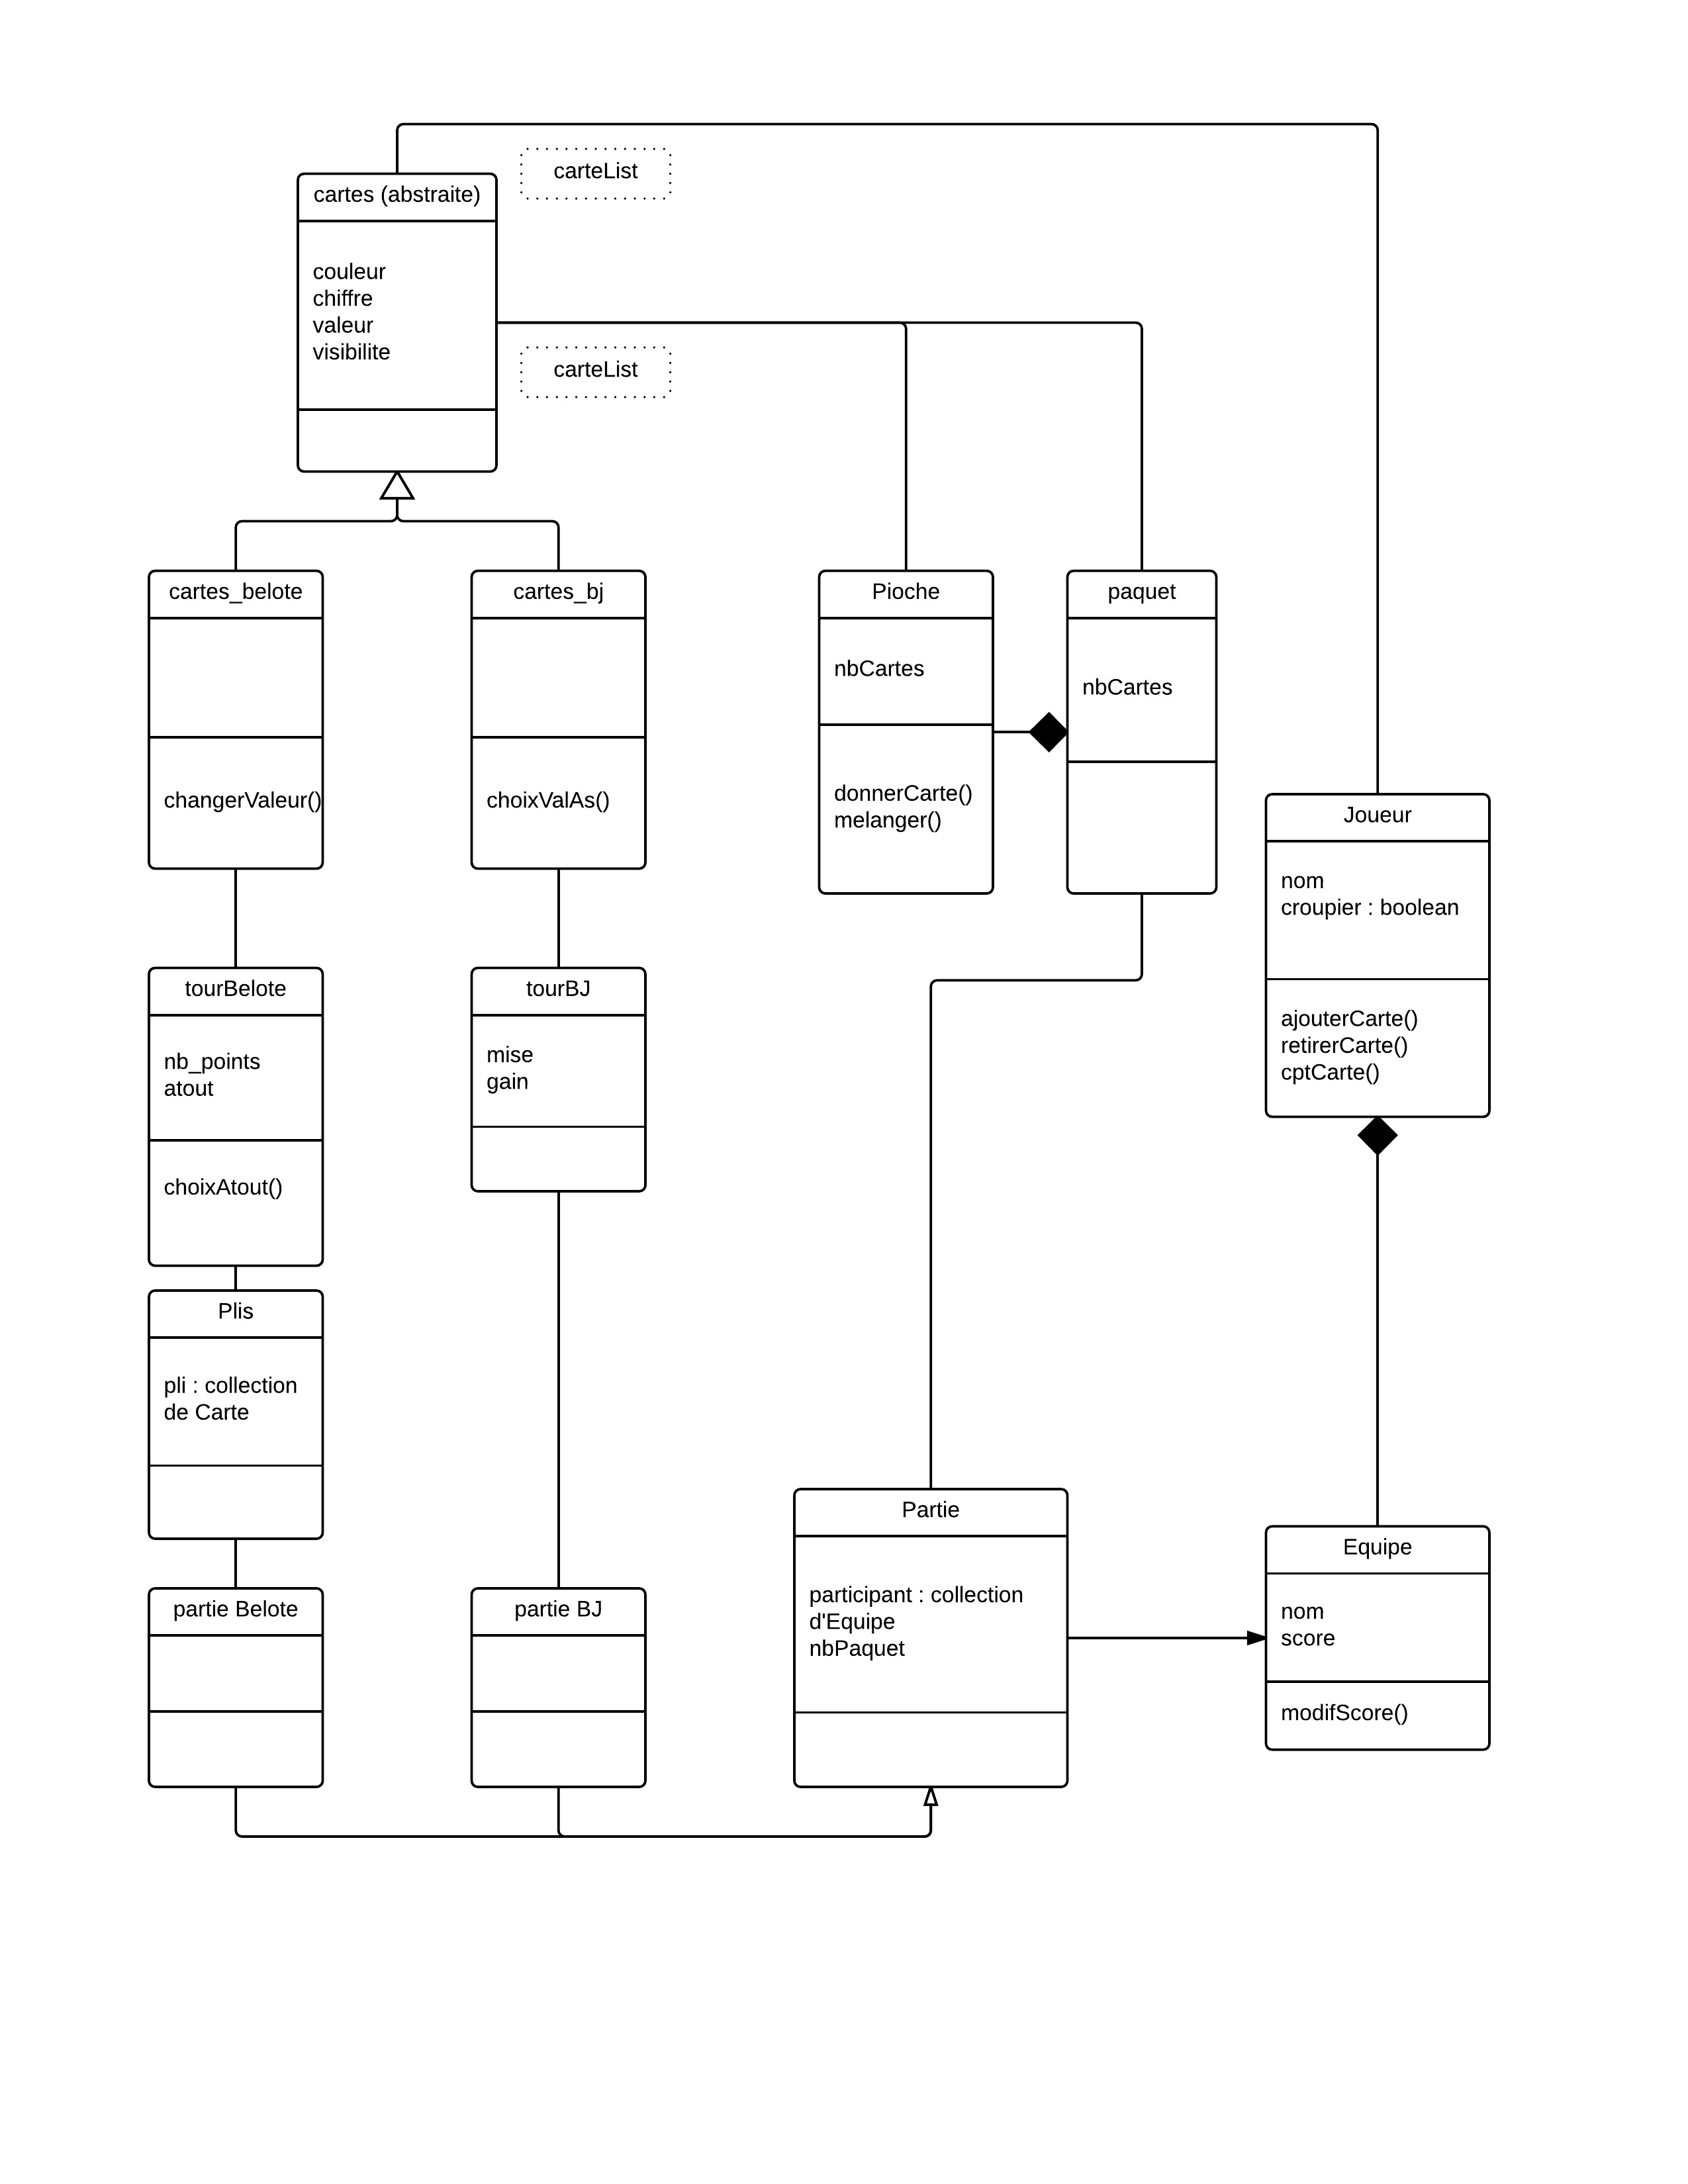
\includegraphics[scale=0.6]{firstUML}
\end{center}

\newpage
\subsubsection{UML final}
\begin{center}
	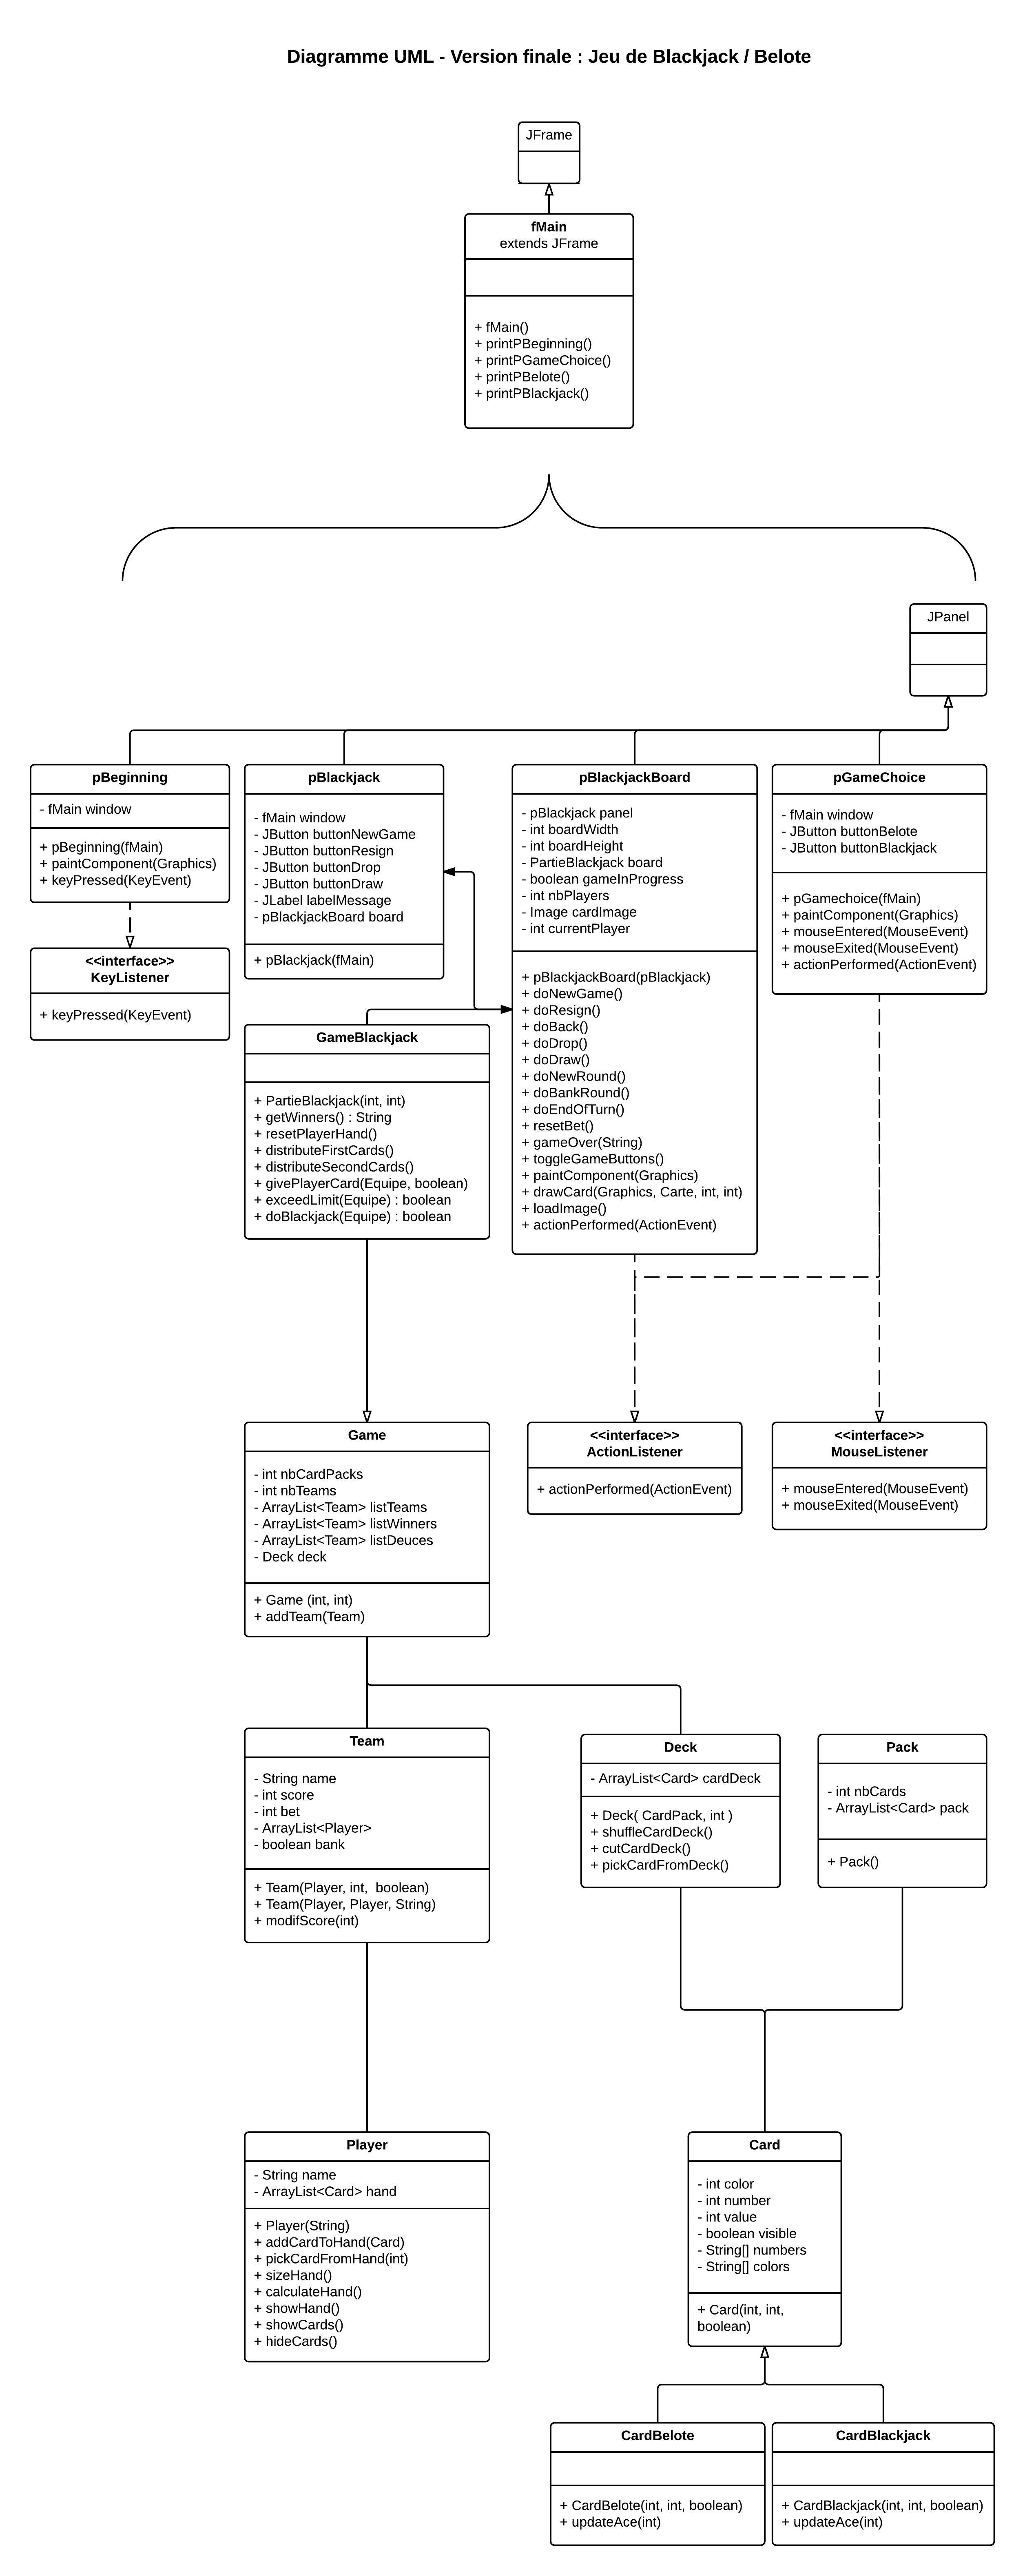
\includegraphics[scale=0.5]{finalUML}
\end{center}

\newpage
\section{Réalisation}
Cela représente un gros volume horaire, que nous n'avons pas compté. Nous avons commencé par créer rapidement les classes communes aux deux jeux (Card, Player, Team, Deck, ...) et qui étaient nécessaires aux classes de déroulement de jeu (Game, GameBelote, GameBlackjack). Une fois faites, nous avons avancé chacun de notre coté, sur nos branches respectives, sur notre jeu.  
\subsection{Liste des classes}
\subsubsection{Classes communes :}
\begin{itemize}
\item \textbf{Application.java} : Simple classe contenant le main et lançant l'application.
\item \textbf{Card.java} : Classe abstraite contenant tous les attributs d'une carte : couleur, valeur et chiffre
\item \textbf{Deck.java} : Pioche, composée d'un ou plusieurs paquets, et qui contient toutes les méthodes dont on pourrait avoir besoin en jeu : couper, mélanger, piocher une carte, etc... Les deux jeux en ont bien évidemment besoin.
\item \textbf{Game.java} : Classe abstraite contenant tous les attributs d'une partie : le nombre d'équipes, le nombre de paquets à utiliser, la liste des gagnants, des perdants, ou des joueurs à égalité.
\item \textbf{IHM.java} : Contient les différents menus pour les jeux, des méthodes d'affichage, de saisie, ... Tout ce qui permet d'interagir avec l'utilisateur, en console.
\item \textbf{Pack.java} : Paquet, il peut contenir 32 ou 52 cartes, il a donc besoin d'un attribut stockant ce nombre, et il contient une Liste de cartes.
\item \textbf{Player.java} : Un Joueur est défini par son nom, et par une main de cartes (liste)
\item \textbf{Team.java} : Une équipe a un score (correspondant à la balance au Blackjack), elle est définie par un nom, et contient des joueurs. Elle stocke aussi l'attribut booléan \textit{bank} pour le Blackjack. L'attribut \textit{bet} retient la mise de l'équipe, pour le Blackjack.
\end{itemize}
Comme on peut le voir ci-dessus, nous avons employé une stratégie un peu particulière. Même si au Blackjack, un score et une mise appartiennent à un joueur, nous avons préféré stocker ces attributs dans la classe Team. En effet, à la Belote, un score correspond à une équipe, et non à un joueur ; nous avons donc choisi de nous aligner avec la Belote pour le Blackjack, en factorisant cet attribut dans la classe Team. Aussi, pour plus de facilité par la suite, nous avons préféré stocker l'attribut \textit{bank} dans la classe Team, plutôt que dans Player.

\subsubsection{Classes Blackjack :}
\begin{itemize}
\item \textbf{CardBlackjack.java} : Cette classe hérite de la classe Card. Elle possède une méthode en plus, permettant de changer la valeur de l'As, soit 1, soit 11pts. Elle permet aussi, dans son constructeur, d'assigner la valeur adéquate à la carte ; comportement différent à la Belote puisque les cartes n'ont pas la même valeur selon le chiffre.
\item \textbf{GameBlackjack.java} : Cette grosse classe rassemble toutes les règles du jeu ; déterminer le(s) gagnant(s) d'un tour, réinitialiser les mains des joueurs, distribuer une carte à une joueur, distribuer les cartes en début de tour, savoir si le joueur a fait un BlackJack ou non ( 21 pts en 2 cartes), ...
\end{itemize}

\subsubsection{Classes Belote :}
\begin{itemize}
	\item \textbf{CardBelote.java} : Comme la classe \textit{CardBelote}, cette classe hérite de la classe Card. La différence avec une carte de Blackjack se situe dans la valeur des cartes qui ne correspondent pas à leur chiffre. De plus, elle possède une méthode lui permettant de changer la valeur des cartes selon si ce sont des cartes d'atout ou non.
	\item \textbf{Trick.java} : Cette classe permet de gérer les plis qui sont effectués à la Belote. Elle dispose d'une méthode permettant de calculer le nombre de points que vaut le pli.
	\item \textbf{GameBelote.java} : Cette classe regroupe l'ensemble des règles de la Belote ; distribuer les cartes, choisir l'atout, savoir qui remporte le pli, et surtout, savoir si un joueur a le droit de poser telle ou telle carte.
\end{itemize}

\subsubsection{Classes graphiques :}
Les classes graphiques se décomposent en 3 catégories :\\
- Frames : fXXXX.java : Fenêtres s'affichant à l'écran, containers des panels\\
- Panels : pXXXX.java : Remplissent les fenêtres et contiennent les différents composants\\
- Listener : XXXXListener.java : Interface réagissant aux événements d'un composant\\
\begin{itemize}
\item \textbf{fMain.java} : Fenêtre principale, dans laquelle se déroule toute l'application, elle s'occupe d'appeler et de dessiner chacun des panels.
\item \textbf{fHandBelote.java} : Fenêtre secondaire qui affiche la main d'un joueur à la Belote.
\item \textbf{pBeginning.java} : Panel protagoniste, n'affichant qu'une image et attendant que l'utilisateur appuie sur Entrée pour passer à l'écran suivant.
\item \textbf{pBelote.java} : Panel principal pour la Belote ; il contient tous les composants (Boutons, Label, ...) et il contient le plateau de jeu, représenté par pBeloteBoard. Il place chacun de ces composants dans la fenêtre et instancie un nouveau plateau.
\item \textbf{pBeloteBoard.java} : Plateau de jeu du Blackjack. Tout le gros du travail se passe ici. Cette classe gère l'action sur le clic sur les boutons, et le déroulement de la partie. Elle s'occupe d'instancier chacun des composants (Boutons, Label, ... ), de définir leur comportement au clic, ... C'est cette classe qui gère le déroulement de la partie, et qui appelle la classe GameBelote pour les règles du jeu. C'est ici que sont disposées les cartes de chaque joueur (face non visible) ainsi que chacun des plis en train d'être joués. C'est également ici que nous pouvons suivre l'évolution du score à la fin de chaque tour de jeu.
\item \textbf{pHandBelote.java} : Panel qui s'occupe de gérer un par un les joueurs de Belote. C'est ici que seront affichées les mains de joueurs (face visible). C'est également ici que les joueurs choisiront la carte à ajouter au pli.
\item \textbf{pBlackjack.java} : Panel principal pour le Blackjack ; il contient tous les composants ( Boutons, Label, ...) et il contient le plateau de jeu, représenté par pBlackjackBoard. Il place donc chacun de ces composants dans la fenêtre et instancie un nouveau plateau.
\item \textbf{pBlackjackBoard.java} : Plateau de jeu du Blackjack. Tout le gros du travail se passe ici. Cette classe gère l'action sur le clic sur les boutons, et le déroulement de la partie. Elle s'occupe d'instancier chacun des composants (Boutons, Label, ... ), de définir leur comportement au clic, ... C'est cette classe qui gère le déroulement de la partie, et qui appelle la classe GameBlackjack pour les règles du jeu. Elle dessine le plateau en chargeant les images, interagi avec l'utilisateur à divers moments, créé un nouveau jeu, abandonne un jeu en cours, ...
\item \textbf{pGameChoice.java} : Second Panel, permettant à l'utilisateur de choisir entre la Belote ou le Blackjack
\item \textbf{WindowHandListener.java} : Classe permettant d'effectuer des actions suite à un événement de la fenêtre \textit{fHandBelote}. 
\end{itemize}

\subsection{La Belote}
\subsubsection{Analyse}

La Belote est un jeu de carte est un jeu de cartes se jouant à 4 avec un jeu de 32 cartes. Les 4 joueurs sont répartis en 2 équipes de 2 joueurs, chacun des joueurs d'une même équipe se faisant face.\\
Le but du jeu est de réaliser des plis (valants un certain nombre de points selon les cartes qui les composent) et de marquer plus de points que l'équipe adverse.\\
A chaque tour sont distribuées, dans un premier temps, 5 cartes à chaque joueur (un tour à 2 cartes suivi d'un tour à 3, ou inversement). A la suite de cette première distribution, la carte située au dessus du paquet de cartes est retournée au milieu de la table.\\
Un premier tour d'enchère s'effectue donc : les joueurs décident, un par un, s'ils veulent prendre la carte retournée et donc jouer à la couleur de la carte (c'est à dire que l'atout sera la couleur de cette carte). Si un des joueurs choisit de la prendre, l'atout est alors fixé et les enchères sont finies. Sinon, un deuxième tour d'enchères s'en suit. Chaque joueur peut alors choisir la couleur de l'atout selon sa main tout en prenant la carte. Si personne ne prend, la donne est finie et on recommence.\\
Une fois l'atout fixé, on distribue le reste du paquet à raison de 3 cartes par joueurs, sauf pour celui qui a pris, qui en reçoit 2. Chaque joueur se retrouve donc avec 8 cartes en main en début de partie.\\
Le joueur situé à gauche du donneur ouvre alors le jeu. A la fin de chaque pli, c'est le joueur qui le remporte qui ouvre à son tour. A la fin de 8 plis, on compte alors l'ensemble des points de chaque équipe. Selon le score effectué et l'équipe preneuse, le score de chaque équipe évolue. La première équipe à 1000pts (par convention mais le score limite peut changer si les équipes se mettent d'accord en début de partie) remporte la partie.\\
On peut déduire, de ces brèves explications, l'algorithme qui nous a servi de base pour l'implémentation de ce jeu :\\

\begin{lstlisting}
donneur = joueur[2][2] //joueur 2 de l'equipe 2
player = { joueur[1][1], joueur[2][1], joueur[1][2], joueur[2][2] }


/*BOUCLE DE JEU*/

Tant que (equipe[0].score < 1000 ET equipe[1].score < 1000)
	/* BOUCLE DE 1ERE DISTRIBUTION
	Pour i=1 à 4
		distribuer(2, player[i]);
	Fin Pour

	/* BOUCLE DE 2EME DISTRIBUTION
	Pour i=1 à 4
		distribuer(3, player[i]);
	Fin Pour

	retournerCarte();

	/* 1ER TOUR D'ANNONCE (ATOUT = COULEUR DE LA CARTE RETOURNEE)
	i=0
	Tant que (player AND choix != 1) //choix = 0 <=> passer, choix = 1 <=> prendre
		player[i].choix = prendre();
		preneur = i;
		i++;
	Fin Tant Que

	/* SI PERSONNE NE PREND, 2EME TOUR D'ANNONCE (choix de l'atout)
	i=0
	Si choix = 0
		Tant que (player AND choix !=1) 
			Si player[i].choix = prendre()
				atout = player[i].choixAtout()
				Pour k= 1 à 4
					Si (k != i)
						distribuer(3, player[k]);
					Sinon
						distribuer(2, player[k]);
					Fin Si
				Fin Pour
			preneur = i;
			i++;
		Si choix = 0
			Nouveau_Tour();
		Fin Si

	Rang = 0 // Pour chaque tour on récupère la place dans le tableau de Joueurs de celui qui prend la main, ainsi le joueur suivant sera player[(rang+1)%4]
	Pour i = 1 à 8
		max = 0;
		Pour j = 1 à 4
			carte = player[(rang+j)%4].poser();
			pli.ajouter(carte);
			Si carte.val > max
				max= carte.val;
				rang = (rang+j)%4;
			Fin Si
		Fin Pour

		pli.val = somme(pli.carte.val)

		Si rang % 2 == 0 //joueur0 ou 2 --> equipe[0]
			pliEquipe0.score += pli.val
		Sinon
			pliEquipe1.score += pli.val
		Fin Si
	Fin Pour

	Si (preneur = 0 ou 2 et pliEquipe0.score <= pliEquipe1.score)
		equipe[0].score += 162;

	Si (preneur = 0 ou 2 et pliEquipe0.score > pliEquipe1.score)
		equipe[0].score += pliEquipe0.score
		equipe[1].score += pliEquipe0.score

	Si (preneur = 1 ou 3 et pliEquipe1.score <= pliEquipe0.score)
		equipe[1].score += 162;

	Si (preneur = 1 ou 3 et pliEquipe1.score > pliEquipe0.score)
		equipe[0].score += pliEquipe0.score
		equipe[1].score += pliEquipe1.score

Fin Tant Que	
\end{lstlisting}

\subsection{Implémentation}
Dans cette partie, nous nous concentrerons sur les méthodes de la classe \textit{GameBelote} car c'est cette classe qui régit l'ensemble des règles du jeu.\\
Afin de pouvoir développer ce jeu aussi bien en console qu'en graphique, il était essentiel de bien découper l'algorithme ci-dessus afin d'avoir un code réutilisable.\\
Tout d'abord, sachant que 2 joueurs côte à côte sont membres d'une équipe différente, il semblait judicieux de 
Ainsi nous retrouvons les méthodes \textit{isValid} et \textit{updateMaster} qui nous permettent respectivement de savoir si le joueur respecte les règles en posant une carte et de stocker le joueur qui est maître (c'est à dire celui qui, au moment où la carte est jouée, va remporter le pli) quand une carte est jouée.


\newpage
\section{Problèmes rencontrés}
\subsection{Git, véritable embouteillage parisien}
\subsection{Penser objet, c'est pas si facile}

\newpage
\section{Conclusion}
\subsection{Le mot de la fin}
\subsection{Bibliographie}
Pour la décomposition en classe et le mécanisme d'un jeu de cartes, en java, nous nous sommes inspirés ici : \\
\url{http://www.apprendre-en-ligne.net/pj/blackjack/chapitre13.pdf}\\\\
Pour apprendre à dessiner une interface graphique, nous nous sommes servis des sources internet suivantes : \\
\url{http://math.hws.edu/javanotes/}\\
\url{http://openclassrooms.com/courses/apprenez-a-programmer-en-java}\\\\
Et nombreuses furent les autres sources : professeurs, camarades, professionnels, ...



\end{document}